\documentclass[a4paper]{article}

\usepackage[utf8]{inputenc}
\usepackage[T1]{fontenc}
\usepackage{algorithm}
\usepackage[noend]{algpseudocode}
\usepackage{amsmath}
\usepackage{amssymb}
\usepackage{amsthm}
\usepackage{graphicx}
\usepackage{stmaryrd}
\usepackage{}

% Define text related commands.
\newcommand{\ie}{\emph{i.e.}}
\newcommand{\eg}{\emph{e.g.}}
\newcommand{\viz}{\emph{viz.}}

\newcommand{\partition}{\pi}
\newcommand{\signature}{\sigma}

\newcommand{\init}{\textsf{init}}
\newcommand{\lts}{\mathcal{L}}
\newcommand{\states}{S}
\newcommand{\actions}{\mathit{Act}}
\newcommand{\semactions}{\Omega}
\newcommand{\action}{a}

\newcommand{\transitions}{\mathbin{\rightarrow}}
\newcommand{\transition}[1]{\xrightarrow{#1}}

\newcommand{\bisim}{\mathbin{\leftrightarroweq}}
\newcommand{\related}{\mathbin{R}}

\newcommand{\set}[1]{\mathcal{P}(#1)}

\newcommand{\refine}{\textsf{refine}}

\renewcommand{\vector}[1]{\langle #1 \rangle}
\newcommand{\var}[1]{\textit{#1}}
\newcommand{\variables}{\mathcal{V}}
\newcommand{\varof}[1]{\textsf{var}(#1)}

\newcommand{\nats}{\mathbb{N}}
\newcommand{\booleans}{\mathbb{B}}

\newcommand{\emptylist}{\ensuremath{[\:]}}
\newcommand{\interpret}[1]{\llbracket #1 \rrbracket}

\newtheorem{theorem}{Theorem}
\newtheorem{lemma}[theorem]{Lemma}
\newtheorem{definition}[theorem]{Definition}
\newtheorem{example}[theorem]{Example}

\title{Symbolic Bisimulation with List Decision Diagrams}
\author{Maurice Laveaux}

\begin{document}

\maketitle
\section{Introduction}

First, we recall several important definitions used in this report.
Let $\actions$ be the set of action \emph{labels}.

\begin{definition}
  A labelled transition system, abbreviated LTS, is a tuple $\lts = (\states, \init, \transitions)$ where $\states$ is a set of states; $\init \in \states$ and $\transitions\,\subseteq \states \times \actions \times \states$ is a labelled transition relation.
\end{definition}

We typically use $\action$, $b$ to denote elements of $\actions$ and we write $s \transition{\action} t$ whenever $(s, \action, t) \in \transitions$.
As usual, a finite LTS can be depicted as an edge-labelled directed graph, where vertices represent states, the labelled edges represent the transitions.

We recall the well-known strong bisimulation equivalence relation on states of an LTS~\cite{Milner83}.

\begin{definition}
  Let $\lts = (\states, \actions, \transitions)$ be an LTS.
  A binary relation $R \subseteq \states \times \states$ is a \emph{(strong) bisimulation relation} iff for all $s \related t$:
  \begin{itemize}
 		\item if $s \transition{\action} s'$ then there is a state $t' \in \states$ such that $t \transition{\action} t'$ and $s' \related t'$, and
 		
 		\item if $t \transition{\action} t'$ then there is a state $s' \in \states$ such that $s \transition{\action} s'$ and $s' \related t'$.
  \end{itemize}

  \noindent
  States $s$ and $t$ are \emph{bisimilar}, denoted $s \bisim t$, iff $s \related t$ for a bisimulation relation $\related$.
\end{definition}

\section{Signature-based Partition Refinement}

One algorithm to compute bisimilarity is based on so-called signature refinement~\cite{WimmerHHSB06}.
Consider any LTS $\lts = (\states, \actions, \transitions)$.

\begin{definition}
  Given a set $S$ then a set of subsets $\partition \subseteq \set{\states}$ is a \emph{partition} iff:
  \begin{equation*}
    \bigcup_{C \in \partition} C = \states \quad \land \quad \forall C, C' \in \partition : (C \neq C') \implies C \cap C' = \emptyset
  \end{equation*}
\end{definition}


\begin{definition}
  Given partitions $\partition$ and $\partition'$ we define $\partition \sqsubseteq \partition'$ iff:
  \begin{align*}
    \forall C \in \partition : \exists C' \in \partition' : C \subseteq C'
  \end{align*}
\end{definition}

\begin{definition}
  A \emph{signature} is a function $\signature : \set{\set{\states}} \times \states \rightarrow T_\signature$, where the sort $T_\signature$ depends on the signature.
\end{definition}

Signature based refinement is now repeatedly refining the partition according to the signature such that states with different signatures end up in different sets of the partition.
Given a signature and a partition we define the following procedure that refines the partition once.
\begin{definition}
  Given a signature $\signature$ and partition $\partition$ we define the refinement function $\refine : \set{\set{\states}} \times \set{\states} \rightarrow \set{\states}$ as follows:
  \begin{equation*}
    \refine(\signature, \partition) = \{ \{ t \in S \mid \signature(\partition, t) = \signature(\partition, s) \} \mid s \in S \}
  \end{equation*}
\end{definition}
Finally, $\nu Z . \refine(\signature, Z)$, where $\nu$ is the largest fixpoint, \ie, the largest partition $Z$ w.r.t $\sqsubseteq$ such that $Z = \refine(\signature, Z)$.
This is the most refined partition.

\section{Signature-based Strong Bisimulation Minimisation}

For strong bisimulation it is known that the following is a suitable signature.

\begin{definition}
  Let $\lts = (\states, \actions, \transitions)$ be an LTS.
  We define the signature for strong bisimulation $\signature_{\bisim} : \set{\set{\states}} \times \states \rightarrow \actions \times \set{\states}$ as follows:
  \begin{equation*}
    \signature_{\bisim}(\partition, s) =  \{ (a, C) \mid \exists C \in \partition, s' \in C: s \transition{a} s' \}
  \end{equation*}
\end{definition}

It holds that $\nu Z . \refine(\signature_{\bisim}, Z)$ is a partition $\partition$ such that the corresponding relation $\related$, where $s \related t$ iff $s, t \in C$ for some $C \in \partition$, is the largest strong bisimulation.
In the following sections we present the a signature based refinement technique using symbolic representations, presented in~\cite{DijkP18}.  

\section{Multi-valued Decision Diagrams}

The set of states of an LTS is typically a set of vectors for the state spaces that we consider.
We denote a \emph{vector} of length $n+1$ by $\vec{d} = \vector{d_0, \ldots, d_n}$.
These set of vectors can be efficiently represented by a so-called decision diagram based on function decomposition.
This representation allows for maximally sharing equivalent sets as well as share prefixes.
Furthermore, it allows for efficient implementation of various set and relational operations that are needed in the actual algorithm.

A set of vectors can be represented by the following function similar to how $\nats \rightarrow \booleans$ represents a set of natural numbers.

\begin{equation*}
  f: \nats \times \cdots \times \nats \rightarrow \booleans
\end{equation*}

We can assume that all process parameters are bounded natural numbers since we can always bidirectionally map from natural numbers to abstract data types.
Now, the we can decompose $f$ on the first argument as follows.

\begin{equation*}
  f(x_0, \ldots, x_n) = 
  \begin{cases}
    f'_0(x_1, \ldots, x_n) &\textsf{if } x_0 = 0 \\
    f'_1(x_1, \ldots, x_n) &\textsf{if } x_0 = 1 \\
    \cdots \\
    f'_{|x_0|}(x_1, \ldots, x_n) &\textsf{if } x_0 = |x_0| \\
  \end{cases}
\end{equation*}

Such that $f(x_0, x_1, \ldots, x_n) = f'_{x_0}(x_1, \ldots, x_n)$ for all $0 \leq x_0 \leq |x_0|, \ldots, 0 \leq x_n \leq |x_n|$, where $|x_0|$ indicates the maximum value of $x_0$.

The decision diagram for this decomposed function consists of vertices and edges where vertices represent the functions, such as $f$ and $f'_0$, and edges the decisions, for example $x_0 = 0$. 
The vertices are maximally shared such that if $f'_0 = f'_1$ then there is a unique vertex in memory representing this function. 
Furthermore, we always decompose on the first argument, so the decision diagram is a tree of height $n+1$.

The resulting decision diagram is called a quasi-reduced multi-valued decision diagrams, which is quasi-reduced since every path from the root to a leaf is exactly $n+1$ long, meaning that it never skips levels. 
For the implementation we use Sylvan [3], which implements list decision diagrams. 
These are unfolded multi-valued decision diagrams where every vertex has exactly two edges, one being the decision and the other being the next element in the list.

\subsection{List Decision Diagrams}

A List Decision Diagram (LDD) is a DAG. It has two types of leaf nodes, \textsf{false} and \textsf{true}, or 0 and 1. The third type of node has a label $a$ and two successors \var{down} and \var{right}, or $=$ and $>$.
An LDD represents a set of lists, as follows:

\begin{equation*}
\begin{array}{lll}
  \llbracket \textsf{false} \rrbracket & = & \emptyset \\
  \llbracket \textsf{true} \rrbracket & = & \{ \emptylist \} \\
  \llbracket \textsf{node}(v, \var{down}, \var{right}) \rrbracket & = & 
    \{ vx \mid x \in \llbracket \var{down} \rrbracket \} \cup \llbracket \var{right} \rrbracket
\end{array}
\end{equation*}

\noindent
In \cite{MeijerBlomPol2008} an LDD is defined as

\begin{definition}
A List decision diagram (LDD) is a
directed acyclic graph with the following properties:
\begin{enumerate}
    \item There is a single root node and two terminal nodes 0 and 1.
    \item Each non-terminal node $p$ is labeled with a value $v$, denoted by $val(p) = v$,
and has two outgoing edges labeled $=$ and $>$ that point to nodes denoted by
$p[x_i = v]$ and $p[x_i > v]$.
    \item For all non-terminal nodes $p$, $p[x_i = v] \neq 0$ and $p[x_i > v] \neq 1$.
    \item For all non-terminal nodes $p$, $val(p[x_i > v]) > v$.
    \item There are no duplicate nodes.
 \end{enumerate}
\end{definition}

\noindent
LDDs are well suited to store lists that differ in only a few positions.
Consider the transition relation $R$ on $S = \mathbb{N}^{10}$ with initial state
$x = [0, 0, 0, 0, 10, 0, 0, 0, 0, 0, 0]$, that is defined by

\[
\textsf{if } x_5 > 0 \textsf{ then begin } x_5 := x_5 - 1; x_6 := x_6 + 1 \textsf{ end}
\]

Clearly this is a sparse relation with $\textsf{used}(R) = \{ 5, 6 \}$. The state space
consists of 11 states that differ only in the 5th and 6th parameter. It can be compactly
represented using an LDD, see the figure below. For our applications we use the LDD implementation that is part of the Sylvan multi-core framework for decision diagrams, see
\cite{DBLP:journals/sttt/DijkP17}.

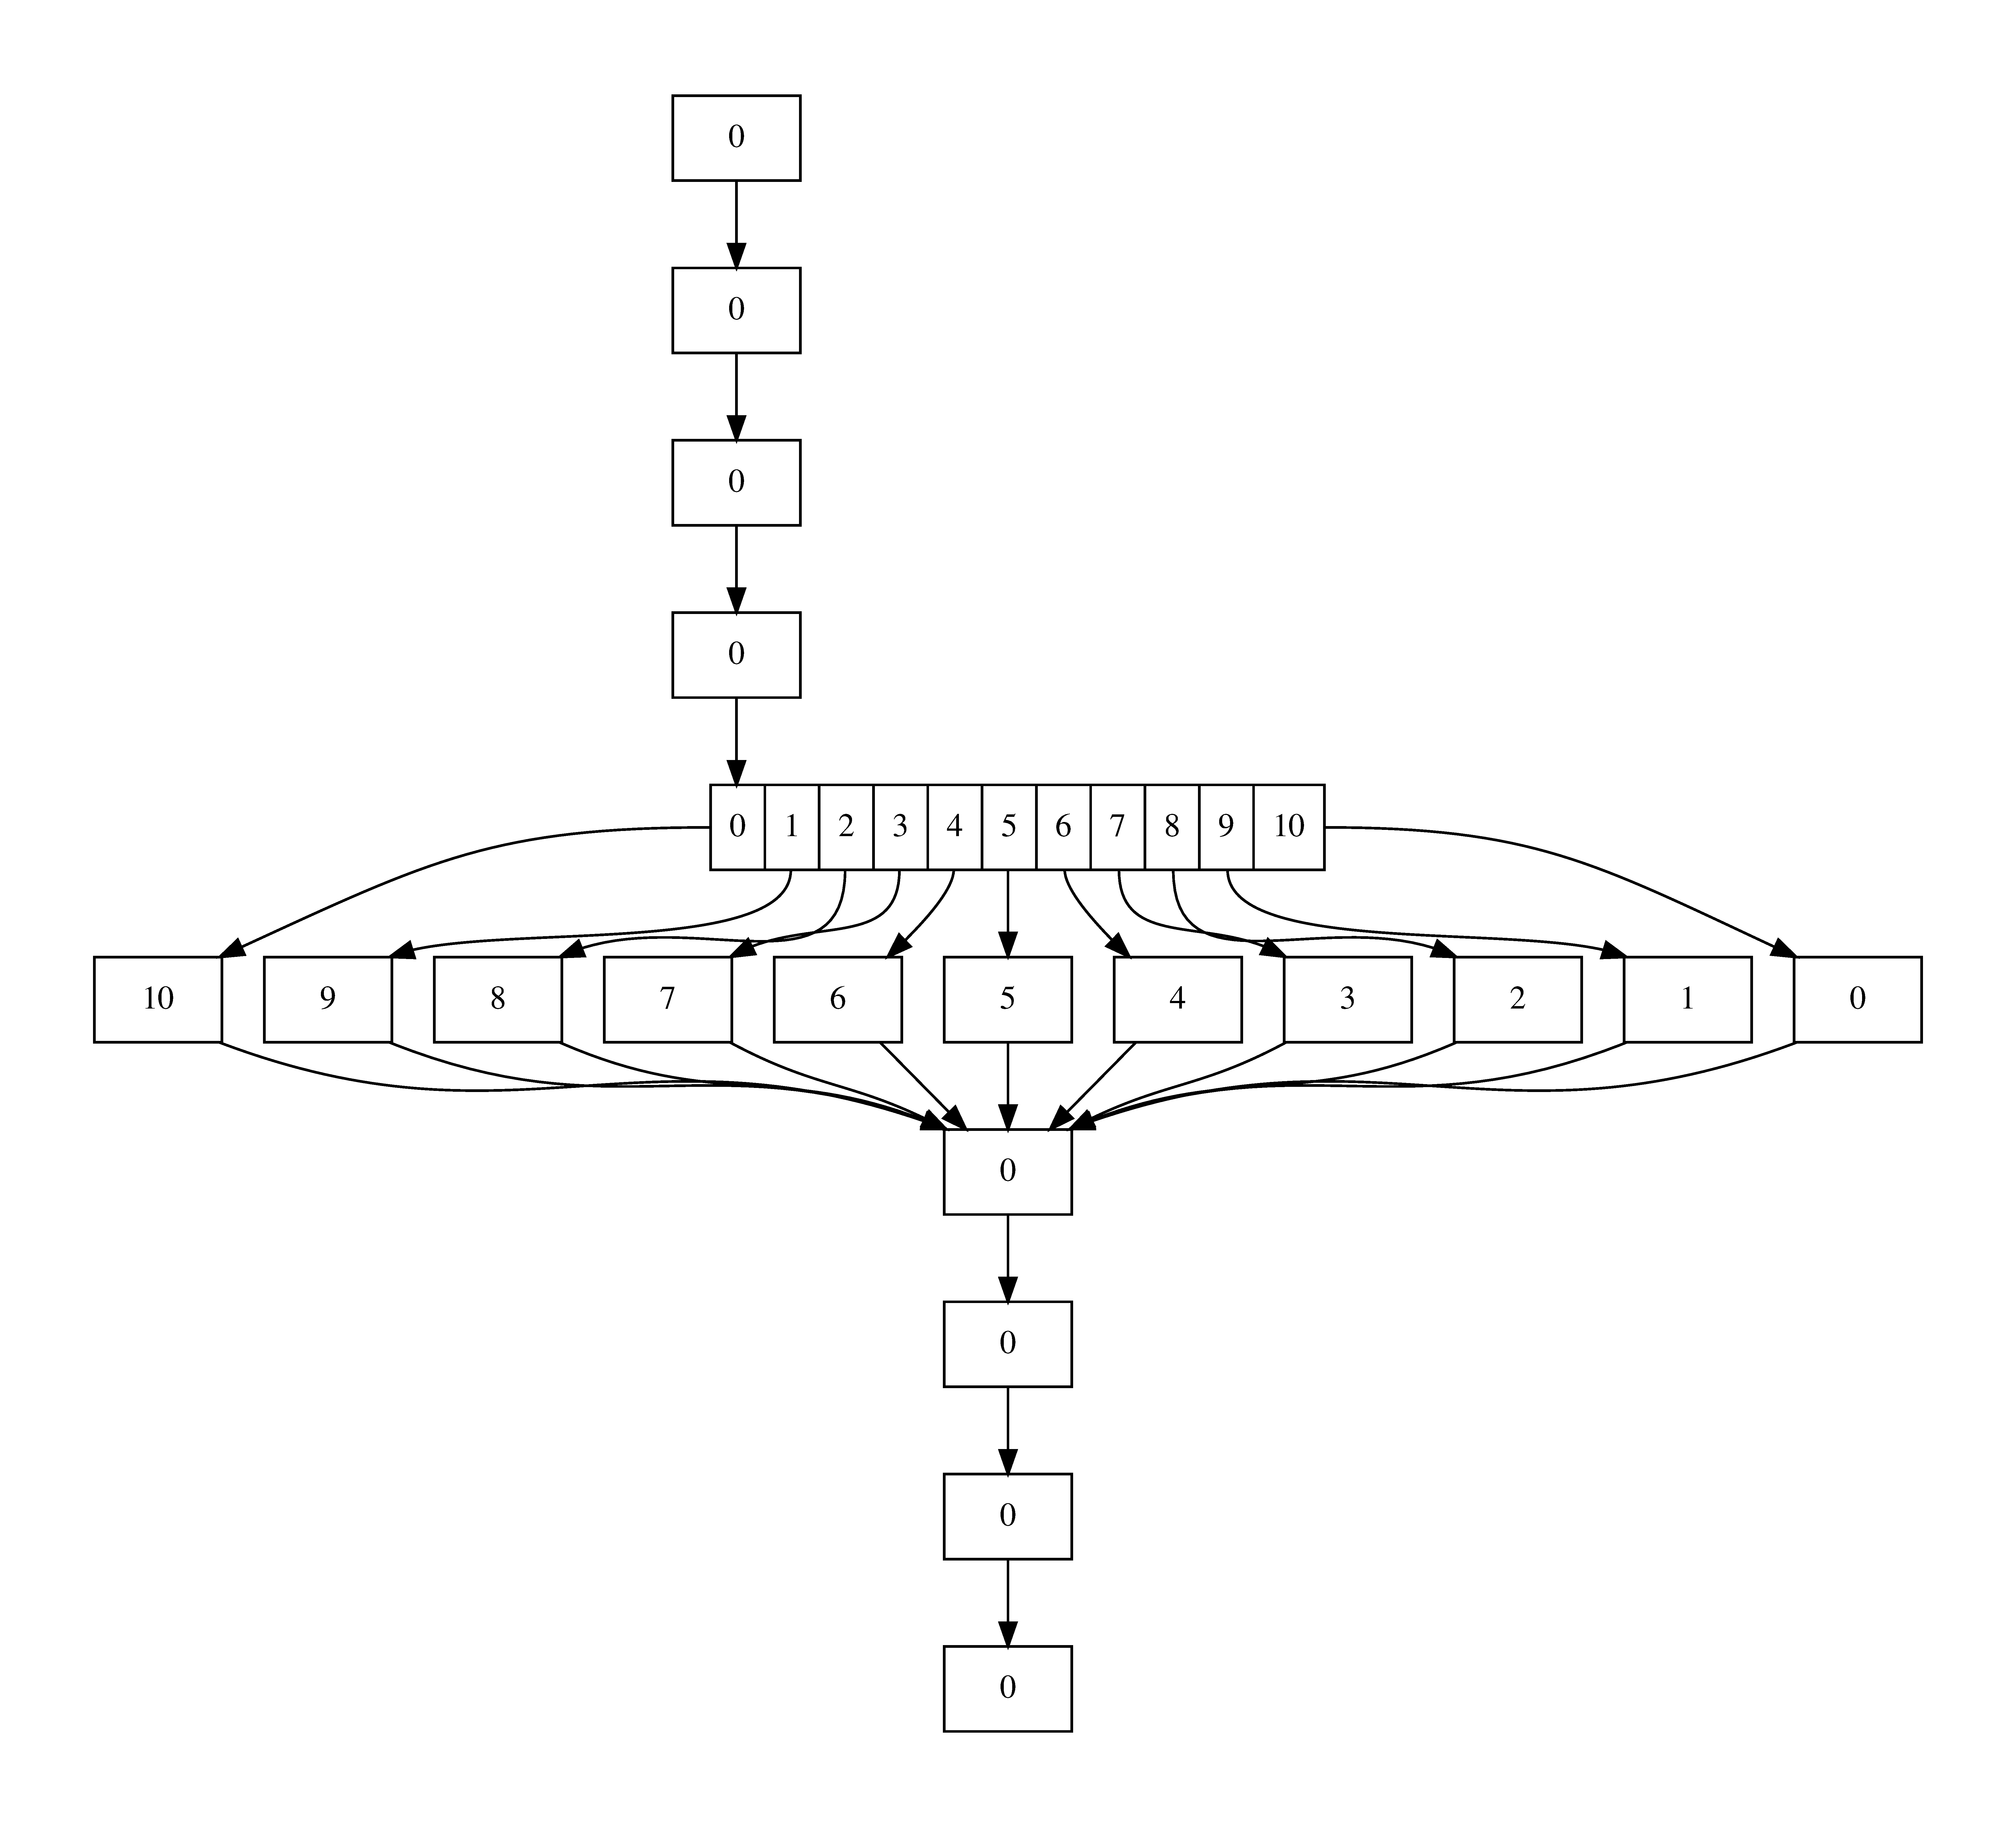
\includegraphics[width=15cm]{ldd_if_then.pdf}

\subsection{Binary Decision Diagrams}

Instead of a vector of natural numbers we can also consider the following specialisation where the input parameters are all booleans.

\begin{equation*}
  f: \booleans \times \cdots \times \booleans \rightarrow \booleans
\end{equation*}

Let $\variables$ be a set of ordered variables.


\subsection{LDD Operations}

There are several options on LDDs that are useful.

The \emph{height} of an LDD is the length from the root to a leaf, because LDDs are quasi-reduced all paths have the same length.


\newcommand{\lddnode}{\textsf{node}}
\newcommand{\lddright}{\textit{right}}
\newcommand{\ldddown}{\textit{down}}
\newcommand{\lddval}{\textit{val}}
\newcommand{\lddtrue}{\textsf{true}}
\newcommand{\lddfalse}{\textsf{false}}

For an LDD $A$ we use $\ldddown(A)$ to denote $A[x_i = v]$ and $\lddright(A)$ to denote $A[x_i > v]$.
We use $|A|$ to denote the size of the LDD, determined by the number of nodes.
Given a vector $v = x_0\,x_1 \cdots x_n$ we define its length, denoted by $|v|$, as $n + 1$.
Note that an LDD can represent (some) sets where two vectors have different lengths.
For example the set $\{1\,1, 0\}$ can be represented by an LDD.
However, the set $\{1\,1, 1\}$ cannot be represented since the root node can either have $\textsf{true}$ or $\var{node}(1, \textsf{true}, \textsf{false})$ as the down node and $\textsf{true}$ has no down or right nodes.
In general, we cannot represent a set with vectors that are strict prefixes (any vector $x_0 \cdots x_m$ with $m < n$ is a strict prefix of $v$) of other vectors in the set.
In practice, this means that we only consider LDDs where every vector in the represented set has the same length.
We refer to this length as the height of the LDD.
We often require that the input LDDs have equal height since not every output can be represented.
For example the union of $\{1\,1\}$ and $\{1\}$ cannot be represented as previously shown.

\subsection{Union}

We define the union operator on two equal height LDDs $A$ and $B$.
This computes the union of the represented sets of vectors.

\begin{algorithm}[h]
\caption{Union of two equal height LDDs $\var{A}$ and $\var{B}$}
\begin{algorithmic}[1]
\Function{union}{$A, B$}
\If{$A = B$}
	\State \Return $a$
\ElsIf{$A = \textsf{false}$}
	\State \Return $b$
\ElsIf{$B = \textsf{false}$}
	\State \Return $a$
\EndIf

\If{$val(A) < val(B)$}
	\State \Return $node(val(A), down(A), \textsc{union}(right(A), B))$
\ElsIf{$val(A) = val(B)$}
	\State \Return $node(val(A), \textsc{union}(down(A), down(B)), \textsc{union}(\lddright(A), right(B)))$
\ElsIf{$val(A) > val(B)$}
	\State \Return $node(val(B), down(B), \textsc{union}(A, right(B)))$	
\EndIf

\EndFunction
\end{algorithmic}
\end{algorithm}

\begin{lemma}
	For all LDDs $A$ and $B$ it holds that $\interpret{\textsc{union}(A, B)} = \interpret{A} \cup \interpret{B}$.
\end{lemma}
\begin{proof}
	Pick arbitrary LDDs $A$ and $B$.
	Proof by induction on the structure of $A$ and $B$.	
	For all LDDs $A'$ and $B'$ we assume that $\interpret{\textsc{union}(A', right(B'))} = \interpret{A'} \cup \interpret{right(B')}$ and $\interpret{\textsc{union}(A', down(B'))} = \interpret{A'} \cup \interpret{down(B')}$.
	Furthermore, $\interpret{\textsc{union}(\var{right}(A'), B')} = \interpret{\var{right}(A')} \cup \interpret{B'}$ and $\interpret{\textsc{union}(down(A'), B')} = \interpret{\var{down}(A')} \cup \interpret{B'}$.
	
	Base case.
	The LDD $A$ is either $\textsf{true}$ or $\textsf{false}$.
	Then $B$ is either $\textsf{true}$ or $\textsf{false}$ due to the equal height assumption.
	In both cases t he terminal conditions ensure correctness.
	For example $\interpret{\textsc{union}(\textsf{true}, \textsf{false})} = \interpret{\textsf{true}}$ and $\{[]\} \cup \emptyset = \{[]\}$.	
	Similarly, for the case where $B$ is either $\textsf{true}$ or $\textsf{false}$.
	
	Inductive step.
	\begin{itemize}
	\item Case $val(A) < val(B)$.
		Since $A$ is an LDD we know that $\lddval(A) < \lddval(\lddright(A))$.
		Therefore, we know that $\interpret{node(val(A), down(A), \textsc{union}(right(A), B))}$ is equal to $\{val(A)\,x \mid x \in \interpret{down(A)}\} \cup \interpret{\textsc{union}(right(A), B)}$.
		It follows that $\interpret{\textsc{union}(right(A), B)}$ is equal to $\interpret{right(A)} \cup \interpret{B}$.
		From which we can derive $\interpret{A} \cup \interpret{B}$.

	\item Case $val(A) = val(B)$.
		Since $A$ is an LDD we know that $\lddval(A) < \lddval(\lddright(A))$ and similarly because $B$ is an LDD we know that $\lddval(A) < \lddval(\lddright(B))$.
		Therefore, the following node is valid and $\interpret{node(val(A), \textsc{union}(down(A), down(B)), \textsc{union}(right(A), \var{right}(B)))}$ is equal to  $\{val(A)\,x \mid x \in \interpret{\textsc{union}(down(A), down(B))}\} \cup \interpret{\textsc{union}(right(A), right(B))}$.
		It follows that the interpretation $\{val(A)\,x \mid x \in \interpret{\textsc{union}(down(A), down(B))}$ is equal to $\{val(A)\,x \mid x \in \interpret{down(A)}\} \cup \{val(A)\,x \mid x \in \interpret{down(B)}\}$ and $\interpret{\textsc{union}(right(A), right(B))}$ is equal to $\interpret{(right(A)} \cup \interpret{right(B))}$.
%		From which we can derive $\interpret{right(A)} \cup \interpret{right(B)}$.
	
	\item Case $val(A) > val(B)$.
		Similar to the $val(A) < val(B)$ case.	\qedhere	
	\end{itemize} 
\end{proof}

We can show that $|\textsc{union(A, B)}|$ for any LDDs $A$ and $B$ is at most $|A| + |B|$.
The time complexity of $\textsc{union(A, B)}$ is also of order $\mathcal{O}(|A| + |B|)$.

\subsection{Project}

Given a vector $x_0\,\cdots\,x_n$ and a subset $I \subseteq \mathbb{N}$, we define the \emph{projection}, denoted by $\textit{project}(x_0\,\cdots\,x_n, I)$, as the vector $x_{i_0}, \ldots, x_{i_l}$ for the largest $l \in \mathbb{N}$ such that $i_0 < i_1 < \ldots < i_l \leq n$ and $i_k \in I$ for $0 \leq k \leq l$.
We define the projection operator for an LDD where every vector in the set is projected.
For the LDD operator it is more convenient to specify the indices $I \subseteq \mathbb{N}$ by a vector $x_0\,\cdots\,x_n$ such that for $0 \leq i \leq n$ variable $x_i$ is one iff $i \in I$.
The operator takes an LDD $A$ of height $n$ and a sequence of numbers $x_0\,x_1,\cdots\,x_n$.

\begin{algorithm}[h]
\caption{Project vectors of an LDD $\var{A}$ of height $n$ using a sequence $x_0\,\cdots\,x_n$}
\begin{algorithmic}[1]
\Function{project}{$A, x_0\,x_1\,\cdots\,x_n$}
	\If{$A = \lddtrue$}
		\State \Return $\lddtrue$
	\ElsIf{$A = \lddfalse$}
		\State \Return $\lddfalse$
	\EndIf
	
	\If{$x_0 = 1$}
		\State \Return{$\lddnode(\lddval(A), \textsc{project}(\ldddown(A), x_1\,\cdots\,x_n), \textsc{project}(\lddright(A), x_0\,\cdots\,x_n))$}
	\ElsIf{$x_0 = 0$}
		\State $a \gets A$
		\State $R \gets \lddfalse$
		\While {$a \neq \lddfalse$}
			\State $R \gets \textsc{union}(R, \textsc{project}(\ldddown(a), x_1\,\cdots\,x_n))$
			\State $a \gets \lddright(a)$		
		\EndWhile			
		\State \Return {$R$}
	\EndIf

\EndFunction
\end{algorithmic}
\end{algorithm}

\begin{lemma}
	For all LDDs $A$ and sequences $x_0\,x_1\,\cdots\,x_n $it holds that $\interpret{\textsc{project}(A, x_0\,\cdots\,x_n)}$ is equal to $\{\textit{project}(v, x_0\,\cdots\,x_n) \in \interpret{A}\}$.
\end{lemma}

Note that for a sequence of $|A|$ zeroes $\textsc{project}(A, 0\,\cdots\,0)$ is equal to $\lddtrue$ and for a sequence of $|A|$ ones $\textsc{project}(A, 1\,\cdots\,1)$ is equal to $A$.

\subsection{Caching}

We can speed up LDD operations at the cost of memory by using an operation cache.
For every operation there will be a separate \emph{global} cache, represented by a set, that stores a tuple of the inputs and the output.
We use \emph{global} to emphasize that every recursion sees the latest values stored in the cache.  
For example the $\textsc{union}(A, B)$ operation has a cache $C_\textsc{union}$ and the pseudocode of $\textsc{union}$ is changed such that after the terminal cases first we check whether $\exists R : (A, B, R) \in C_\textsc{union}$ and return the result $R$ if that is the case.
Otherwise, we perform the computation as before but store the result in $C_\textsc{union}$ instead before returning it.
Thus we obtain the following algorithm:

\begin{algorithm}[H]
\caption{Union of two LDDs $\var{A}$ and $\var{B}$.
	With a set $C_\textsc{union}$ as operation cache}
\begin{algorithmic}[1]
\Function{union}{$A, B,  C_\textsc{union}$}
\If{$A = B$}
	\State \Return $a$
\ElsIf{$A = \textsf{false}$}
	\State \Return $b$
\ElsIf{$B = \textsf{false}$}
	\State \Return $a$
\EndIf

\If{$\exists R: (A, B, R) \in C_\textsc{union}$}
	\Return $R$
\EndIf

\If{$val(A) < val(B)$}
	\State $R \gets node(val(A), down(A), \textsc{union}(right(A), B, C_\textsc{union}))$
\ElsIf{$val(A) = val(B)$}
	\State $R \gets node(val(A), union(down(A), down(B), union(right(A), right(B), C_\textsc{union}))$
\ElsIf{$val(A) > val(B)$}
	\State $R \gets node(val(B), down(B), \textsc{union}(A, right(B), C_\textsc{union}))$
\EndIf

\State $C_\textsc{union} \gets C_\textsc{union} \cup \{(A, B, R)\}$
\State \Return $R$
\EndFunction
\end{algorithmic}
\end{algorithm}

\subsection{Parallelism}

In some cases we can improve the performance further by computing several results in parallel during the operation.
For example in the union of two LDDs $A$ and $B$ in the case $val(A) = val(B)$ we could determine the result of both unions in parallel and only merge them after they have finished.


\section{Signature-based Refinement (BDD)}

The variable $\var{blocks}$ is an associative container mapping block numbers to signatures, and has the operations.
We assume that the states are encoded by a BDD over variables $v_0, \ldots, v_n$, and the transitions by a BDD with variables $v'_0 < \ldots < v'_n$

\begin{algorithm}[h]
  \footnotesize
  \caption{Given signature $\signature$ and partition $\partition$ computes $\refine(\signature, \partition)$.}\label{alg:cleave}
  \begin{algorithmic}[1]
    \Procedure{\textsc{Refine-Rec}}{$\signature$, $\partition$, $\var{cache}$, $\var{blocks}$}
      \If{$\partition = \bot$}
        \Return{$\bot$}
      \EndIf
      
      \If{$\exists \alpha: (\signature, \partition, \alpha) \in \var{cache}$}
        \Return{$\alpha$}
      \EndIf
      
      \If{$\varof{\partition} \in \{v_0, \ldots, v_n\}$}
      
      \EndIf
      
      
  
    \EndProcedure
  \Procedure{\textsc{Refine}}{$\signature$, $\partition$}
    \State{$\var{cache} \gets \emptyset$}
    \State{$\var{blocks} \gets \emptyset$}
  

  \EndProcedure
  \end{algorithmic}
\end{algorithm}



\bibliographystyle{plain}
\bibliography{bibliography}

\end{document}